\hypertarget{_number_draw_8cpp}{}\section{C\+:/\+H\+A\+L/\+P\+G関係/03\+\_\+作成プログラム/03\+\_\+\+H\+A\+L授業/就職作品/\+Project/source/04\+\_\+\+Tool/\+Numbers/\+Number/\+Number\+Draw/\+Number\+Draw.cpp ファイル}
\label{_number_draw_8cpp}\index{C\+:/\+H\+A\+L/\+P\+G関係/03\+\_\+作成プログラム/03\+\_\+\+H\+A\+L授業/就職作品/\+Project/source/04\+\_\+\+Tool/\+Numbers/\+Number/\+Number\+Draw/\+Number\+Draw.\+cpp@{C\+:/\+H\+A\+L/\+P\+G関係/03\+\_\+作成プログラム/03\+\_\+\+H\+A\+L授業/就職作品/\+Project/source/04\+\_\+\+Tool/\+Numbers/\+Number/\+Number\+Draw/\+Number\+Draw.\+cpp}}
{\ttfamily \#include $<$assert.\+h$>$}\newline
{\ttfamily \#include \char`\"{}Number\+Draw.\+h\char`\"{}}\newline
{\ttfamily \#include $<$Resource\+Manager\textbackslash{}\+Resource\+Manager.\+h$>$}\newline
{\ttfamily \#include $<$Polygon\textbackslash{}\+Plane\+Polygon\textbackslash{}\+Plane\+Polygon.\+h$>$}\newline
Number\+Draw.\+cpp の依存先関係図\+:
\nopagebreak
\begin{figure}[H]
\begin{center}
\leavevmode
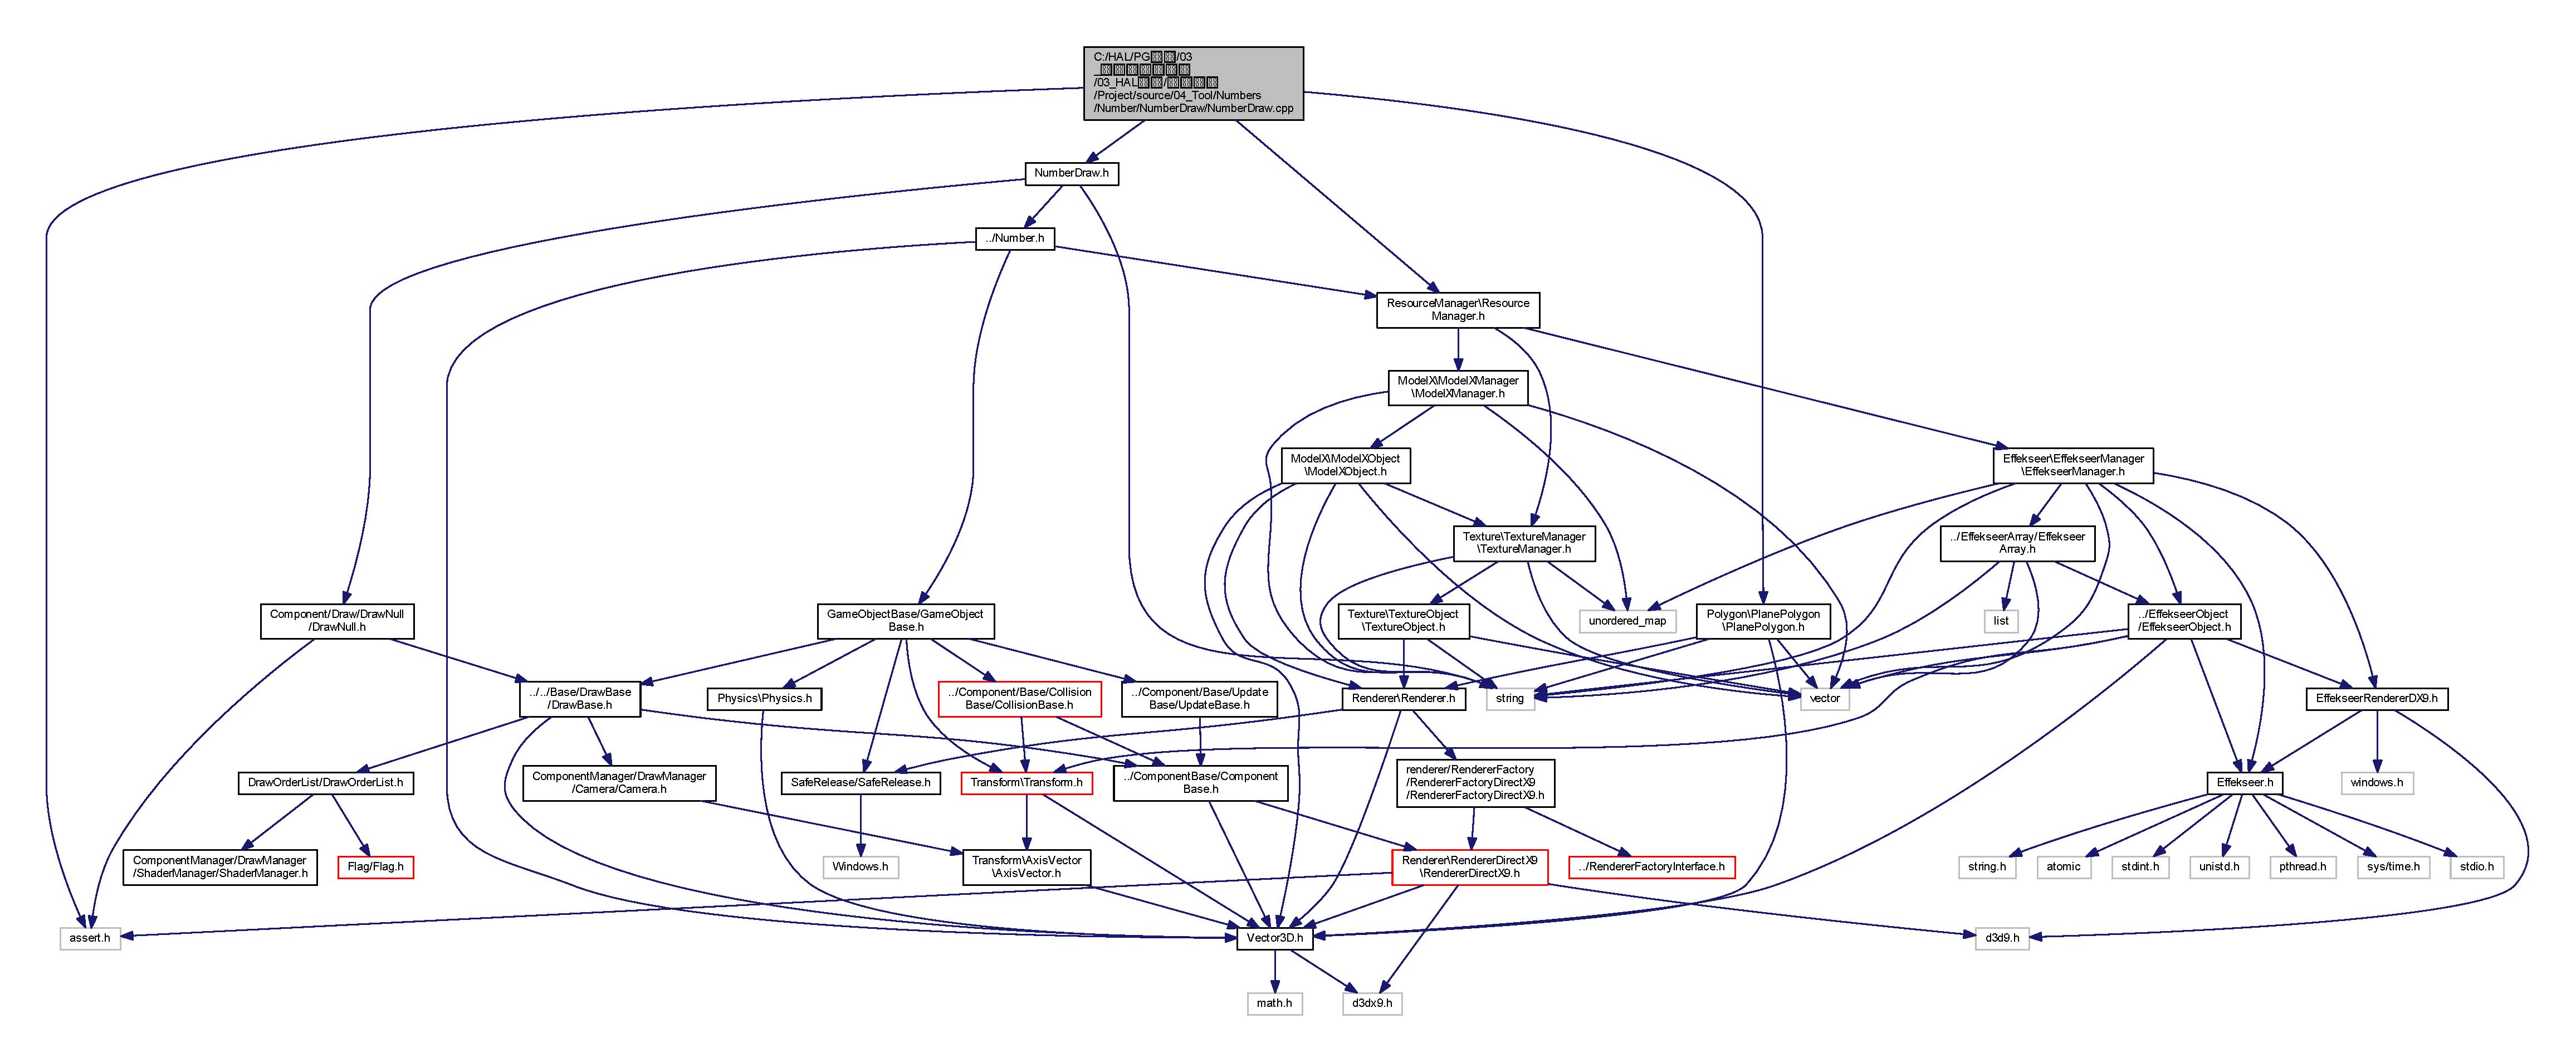
\includegraphics[width=350pt]{_number_draw_8cpp__incl}
\end{center}
\end{figure}
